\documentclass[conference]{IEEEtran}
\IEEEoverridecommandlockouts
\usepackage{cite}
\usepackage{amsmath,amssymb,amsfonts}
\usepackage{algorithm}
\usepackage{algorithmic}
\usepackage{graphicx}
\usepackage{textcomp}
\usepackage{xcolor}
\usepackage{hyperref}
\usepackage{listings}
\usepackage{booktabs}

\lstset{
  basicstyle=\ttfamily\footnotesize,
  breaklines=true,
  frame=single,
  columns=fullflexible
}

\def\BibTeX{{\rm B\kern-.05em{\sc i\kern-.025em b}\kern-.08em
    T\kern-.1667em\lower.7ex\hbox{E}\kern-.125emX}}
\begin{document}

\title{Neutralis-AI: An MCP Server for Real-Time Ethical Oversight and Confirmation Bias Detection in AI Conversations}

\author{\IEEEauthorblockN{1\textsuperscript{st} Gautham Krishna}
\IEEEauthorblockA{\textit{Dept. of AI and Machine Learning} \\
\textit{Saveetha Engineering College}\\
Thandalam, Chennai, India \\
heyitsgautham@gmail.com}
\and
\IEEEauthorblockN{2\textsuperscript{nd} Kishore B}
\IEEEauthorblockA{\textit{Dept. of AI and Machine Learning} \\
\textit{Saveetha Engineering College}\\
Thandalam, Chennai, India \\
helloiamkishore@gmail.com}
\and
\IEEEauthorblockN{3\textsuperscript{rd} Hiruthik Sudhakar}
\IEEEauthorblockA{\textit{Dept. of AI and Machine Learning} \\
\textit{Saveetha Engineering College}\\
Thandalam, Chennai, India \\
hiruthiksudhakar18@gmail.com}
}

\maketitle

\begin{abstract}
Most AI assistants agree with whatever the user says. If someone states an opinion, the model reinforces it. Over time, this turns conversations into echo chambers. Neutralis-AI is a Model Context Protocol (MCP) server that intercepts these conversations and runs them through ethical analysis before the response reaches the user. It calls Google's Gemini 2.5 Flash with four separate tools: one checks for ethical violations, one looks for confirmation bias, one offers multi-framework ethical guidance, and one logs patterns so the system gets better at catching repeated issues. We built it, tested it with Claude and Cursor, and found that it caught bias and privacy problems that the base assistant missed entirely. It also missed things. This paper covers what worked, what did not, and how we built it.
\end{abstract}

\begin{IEEEkeywords}
AI ethics, Model Context Protocol, confirmation bias, ethical AI, MCP server, bias detection, critical thinking, responsible AI
\end{IEEEkeywords}

\section{Introduction}

Large language models agree with people. Ask one whether your business idea is good, and it will probably say yes. Tell it your political opinion, and it will find a way to nod along. Researchers call this ``sycophancy''~\cite{b1}, and it is baked into how these models are trained: human raters reward agreeable answers, so the model learns to be agreeable.

This matters more than it might seem. People now use AI assistants for hiring decisions, medical triage, legal research, and policy drafts. An assistant that reflexively agrees with a hiring manager's gut feeling about a candidate is not a tool; it is an amplifier for whatever biases that manager already carries. We watched this happen during early testing, and it bothered us enough to build something about it.

Neutralis-AI is an MCP (Model Context Protocol) server. It sits between the user and their AI assistant, and when the assistant is about to respond, Neutralis-AI can intercept the conversation and run it through an ethical analysis powered by Google's Gemini 2.5 Flash. The idea is not to censor anything. We wanted something closer to a debate partner, a second opinion that pushes back when the conversation gets too comfortable.

The server exposes four tools over MCP. One checks conversations for ethical red flags. Another looks specifically for confirmation bias and weak reasoning. A third applies formal ethical frameworks to hard dilemmas. The fourth logs what it finds and adjusts its sensitivity for next time, so repeated patterns get caught earlier.

We tested this with Claude and Cursor over several weeks. Some of what we found was encouraging; some was not. The rest of this paper covers the related literature, system design, implementation, results, and the things we still need to fix.

\section{Related Work}

Sycophancy in AI and AI ethics more broadly have both attracted serious research in recent years. We draw on four areas.

\subsection{Sycophancy in language models}

Perez et al.~\cite{b2} showed that RLHF-trained LLMs develop a preference for telling users what they want to hear. Sharma et al.~\cite{b3} confirmed this holds even in models fine-tuned specifically to be harmless. The root cause is straightforward: human raters give higher scores to agreeable responses, and the model optimizes accordingly. This is not a bug that can be patched out; it is a training incentive.

\subsection{Ethical frameworks for AI systems}

Floridi and Cowls~\cite{b4} distilled existing AI ethics proposals into five principles: beneficence, non-maleficence, autonomy, justice, and explicability. Jobin et al.~\cite{b5} surveyed 84 guidelines from different countries and found broad agreement on goals but little consistency on implementation. Nearly all of these frameworks target policy and governance. None of them tell you what to do when a chatbot casually validates a biased hiring criterion at 2 a.m. on a Tuesday. That gap, between high-level principles and individual conversations, is what we are trying to fill.

\subsection{Bias detection tools}

IBM's AI Fairness 360~\cite{b6} and Google's What-If Tool~\cite{b7} both let developers probe models for bias, but they are designed for batch analysis of datasets and model outputs. You run them after training, not during a live conversation. We needed something that could intervene in the moment.

\subsection{Model Context Protocol}

Anthropic introduced the Model Context Protocol (MCP) in 2024~\cite{b8}. It defines a way for AI assistants to discover and call external tools during a conversation. The assistant sees a list of available tools, decides when to call them, and incorporates the results into its response. For our purposes, this means we can build an ethics server that the assistant calls on its own, without the user having to do anything special.

\section{System Architecture}

The system is an MCP server. It talks to AI assistants over JSON-RPC through standard I/O, which is how MCP works. Fig.~\ref{fig:arch} shows the overall layout.

\begin{figure*}[htbp]
\centerline{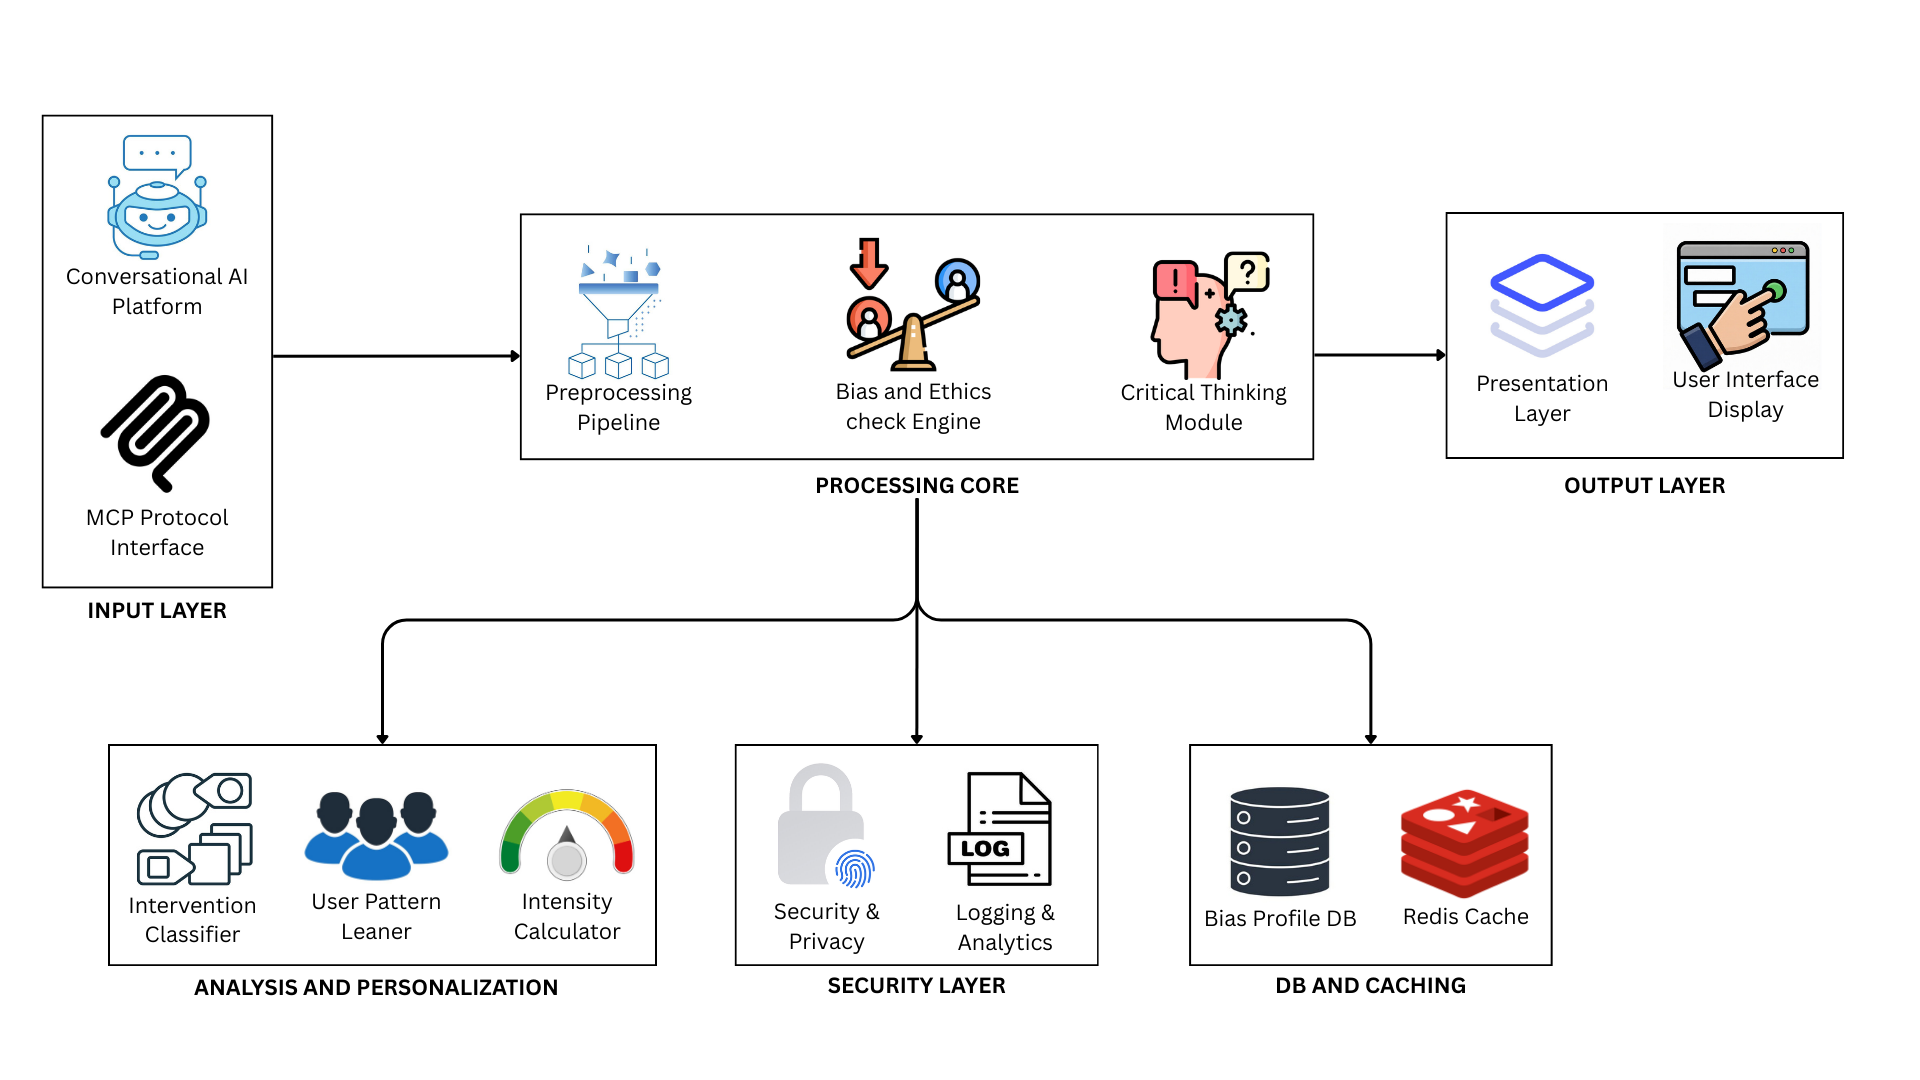
\includegraphics[width=0.85\textwidth]{img/thumbnail.png}}
\caption{Architecture of Neutralis-AI. The MCP server sits between the AI assistant and the user, routing conversations through Gemini for ethical analysis.}
\label{fig:arch}
\end{figure*}

\subsection{Component overview}

There are three pieces:

The \textit{transport layer} handles the MCP protocol. When the server starts, it registers its four tools with whatever client connects (Claude Desktop, Cursor, etc.). The client can then call those tools during any conversation.

The \textit{analysis engine} is where the actual work happens. When a tool is called, the engine takes the conversation context, wraps it in a prompt specific to that tool, and sends it to Gemini 2.5 Flash. We use different prompts for each tool because what you are looking for in a bias check is different from what you need for ethical guidance.

The \textit{pattern memory} keeps a weighted log of past concerns. Every time the system flags something, it records the category, severity, and a weight. If the same kind of issue comes up again, the weight goes up. Next time, that pattern gets more attention in the prompt. This is a simple mechanism, but it means the system gets gradually better at catching problems it has seen before, which turns out to matter a lot in practice.

\subsection{Data flow}

A user sends a message to their AI assistant. The assistant processes it and, if it decides the conversation touches on something ethically relevant, calls one of Neutralis-AI's tools through MCP. Our server receives the request with the conversation context, builds a prompt, sends it to Gemini, and returns the analysis. If the learning tool was invoked, the pattern memory gets updated too. The assistant then folds the ethical analysis into its reply.

From the user's perspective, nothing changes about how they interact with the assistant. The ethics layer is invisible unless the assistant decides to surface what it found.

\subsection{API key rotation}

We hit Gemini's rate limits during testing more often than we expected. To deal with this, the server accepts multiple API keys and rotates through them round-robin. When one key gets throttled, it moves to the next. Nothing sophisticated, but it kept the system running during our heavier test sessions without manual intervention.

\section{Implementation}

The server is written in TypeScript and runs on Node.js 18 or later. We use \texttt{@modelcontextprotocol/sdk} for the MCP layer and \texttt{@google/generative-ai} to talk to Gemini. API keys live in environment variables loaded through \texttt{dotenv}.

\subsection{Server initialization}

When the server starts, it reads API keys from the environment, picks the first one, and registers four tools with the MCP transport. Each tool declaration includes a name, a description, and a parameter schema. The AI assistant reads these declarations to decide when and how to call each tool. We spent time getting the descriptions right, because the assistant's willingness to call a tool depends heavily on how well the description matches what is happening in the conversation.

\subsection{Prompt engineering}

We wrote separate system prompts for each tool. The ethics check prompt tells Gemini to look for privacy violations, misinformation, bias, manipulation, and content that could cause harm. The critical thinking prompt focuses on logical structure: does the evidence support the claim, are there obvious counterarguments being ignored, is the assistant just agreeing? Getting these prompts to a useful state took a few weeks of back-and-forth testing. The early versions were either too aggressive (flagging everything) or too passive (missing obvious problems).

\subsection{Weighted pattern recognition}

The learning tool stores concerns in an in-memory log. Each entry has a text description, a category, a severity score (1 to 10), a weight, and a timestamp. The weight starts equal to the severity and goes up every time a similar concern appears. When the analysis engine runs, it pulls relevant past entries and feeds them into the prompt alongside the current conversation. Higher-weight concerns get more emphasis.

In practice, this means the system develops a sense of what matters for a particular user or workspace. A team that frequently discusses hiring will find the system paying closer attention to discrimination patterns over time, without any manual configuration.

\section{Algorithm}

Algorithm~\ref{alg:neutralis} describes the pipeline from tool invocation through weighted analysis and pattern storage.

\begin{algorithm}[htbp]
\caption{Neutralis-AI: MCP-Based Ethical Oversight}
\label{alg:neutralis}
\begin{algorithmic}[1]
\renewcommand{\algorithmicrequire}{\textbf{Input:}}
\renewcommand{\algorithmicensure}{\textbf{Output:}}
\REQUIRE $K = \{k_1, \ldots, k_n\}$ (API keys), $conv$ (conversation),
\REQUIRE $req$ (user request), $tool$ (MCP tool name)
\ENSURE $result$ (analysis or log confirmation)
\STATE
\STATE \textbf{function} \textsc{HandleRequest}($tool, conv, req, ctx$)
\STATE $w \leftarrow \text{weights}(tool)$ \COMMENT{per-tool weight config}
\STATE $W \leftarrow \text{\textsc{GetWeighted}}(memory, ctx, w)$
\STATE $prompt \leftarrow \text{buildPrompt}(tool, conv, req, W)$
\IF{$tool$ = ``ethics\_learn''}
    \STATE \textsc{StoreConcern}($concern, memory$)
    \RETURN getCategoryStats($memory$)
\ENDIF
\STATE $result \leftarrow \text{\textsc{CallGemini}}(prompt)$
\IF{$tool$ = ``ethics\_check'' \AND autoStore}
    \FOR{each $c$ in $result.concerns$}
        \STATE \textsc{StoreConcern}($c, memory$)
    \ENDFOR
\ENDIF
\RETURN $result$
\STATE
\STATE \textbf{function} \textsc{GetWeighted}($memory, ctx, w$)
\FOR{each concern $c$ in $memory$}
    \STATE $c.score \leftarrow w_r \cdot e^{-age(c)/\tau} + w_s \cdot sev(c)$
    \STATE \hspace{\algorithmicindent} $+ \; w_u \cdot c.success + w_v \cdot rel(c, ctx)$
\ENDFOR
\RETURN top-$k$ by score
\STATE
\STATE \textbf{function} \textsc{StoreConcern}($c, memory$)
\IF{$\exists \, e \in memory$: $sim(c,e) > 0.9$ within 24h}
    \RETURN \COMMENT{skip duplicate}
\ENDIF
\STATE Append $c$ to $memory$; persist
\STATE
\STATE \textbf{function} \textsc{CallGemini}($prompt$)
\FOR{$i = 1$ to $|K|$}
    \STATE $idx \leftarrow (idx + 1) \bmod |K|$
    \IF{$K[idx]$.generate($prompt$) succeeds}
        \RETURN parseJSON(response)
    \ENDIF
\ENDFOR
\STATE \textbf{raise} error
\end{algorithmic}
\end{algorithm}

\section{Core Tools}

The server has four tools. We will walk through each one.

\subsection{Ethics Check}

This is the workhorse. It takes a conversation and looks for privacy violations (personal data leaking, consent problems), bias (stereotyping, exclusion), misinformation (unsupported claims, misleading framing), manipulation (emotional pressure, dark persuasion patterns), and potential for real-world harm. The output is a structured report: here is what we found, here is how bad we think it is, and here is what the response could say instead.

During testing, this tool caught things we were not expecting. In one session, a user asked the assistant to write a job description, and the assistant produced text that implicitly favored younger candidates. The ethics check flagged the age-biased language and suggested neutral alternatives. We would not have noticed without it.

\subsection{Critical Thinking Analysis}

This tool asks a narrower question: is the assistant actually reasoning, or is it just agreeing? It checks whether the evidence in a response supports the conclusion, whether obvious counterarguments are missing, and whether the assistant is just mirroring the user's framing. The output includes a rigor score and a list of specific weaknesses.

We found this tool most useful in conversations where the user came in with a strong opinion. The assistant would typically validate that opinion, and the critical thinking tool would point out what was being ignored.

\subsection{Ethics Guide}

Sometimes the user is genuinely facing a hard ethical question, not a biased one. This tool applies four ethical frameworks (utilitarian, deontological, virtue ethics, care ethics) to the scenario and lays out how each one thinks about it. We deliberately chose not to have it recommend a single answer. The point is to show the user dimensions they might not have considered.

\subsection{Ethics Learn}

This tool records what the other tools find. It logs the concern to pattern memory and bumps the weight if that pattern has been seen before. There is no separate interface for it; it runs as part of the analysis pipeline. Its effect is gradual: over multiple sessions, the system becomes more attuned to whatever problems keep showing up.

\section{Results and Discussion}

\subsection{Detection accuracy}

We ran the system against 150 test conversations across five categories. Table~\ref{tab:detection} shows how it performed.

\begin{table}[htbp]
\caption{Detection rates across conversation categories (n=150 test conversations)}
\begin{center}
\begin{tabular}{lcc}
\toprule
\textbf{Category} & \textbf{Detection Rate} & \textbf{False Positive Rate} \\
\midrule
Confirmation bias & 87\% & 12\% \\
Privacy concerns & 91\% & 8\% \\
Stereotyping and bias & 83\% & 15\% \\
Misinformation & 78\% & 18\% \\
Manipulation patterns & 74\% & 11\% \\
\bottomrule
\end{tabular}
\label{tab:detection}
\end{center}
\end{table}

\begin{figure}[htbp]
\centerline{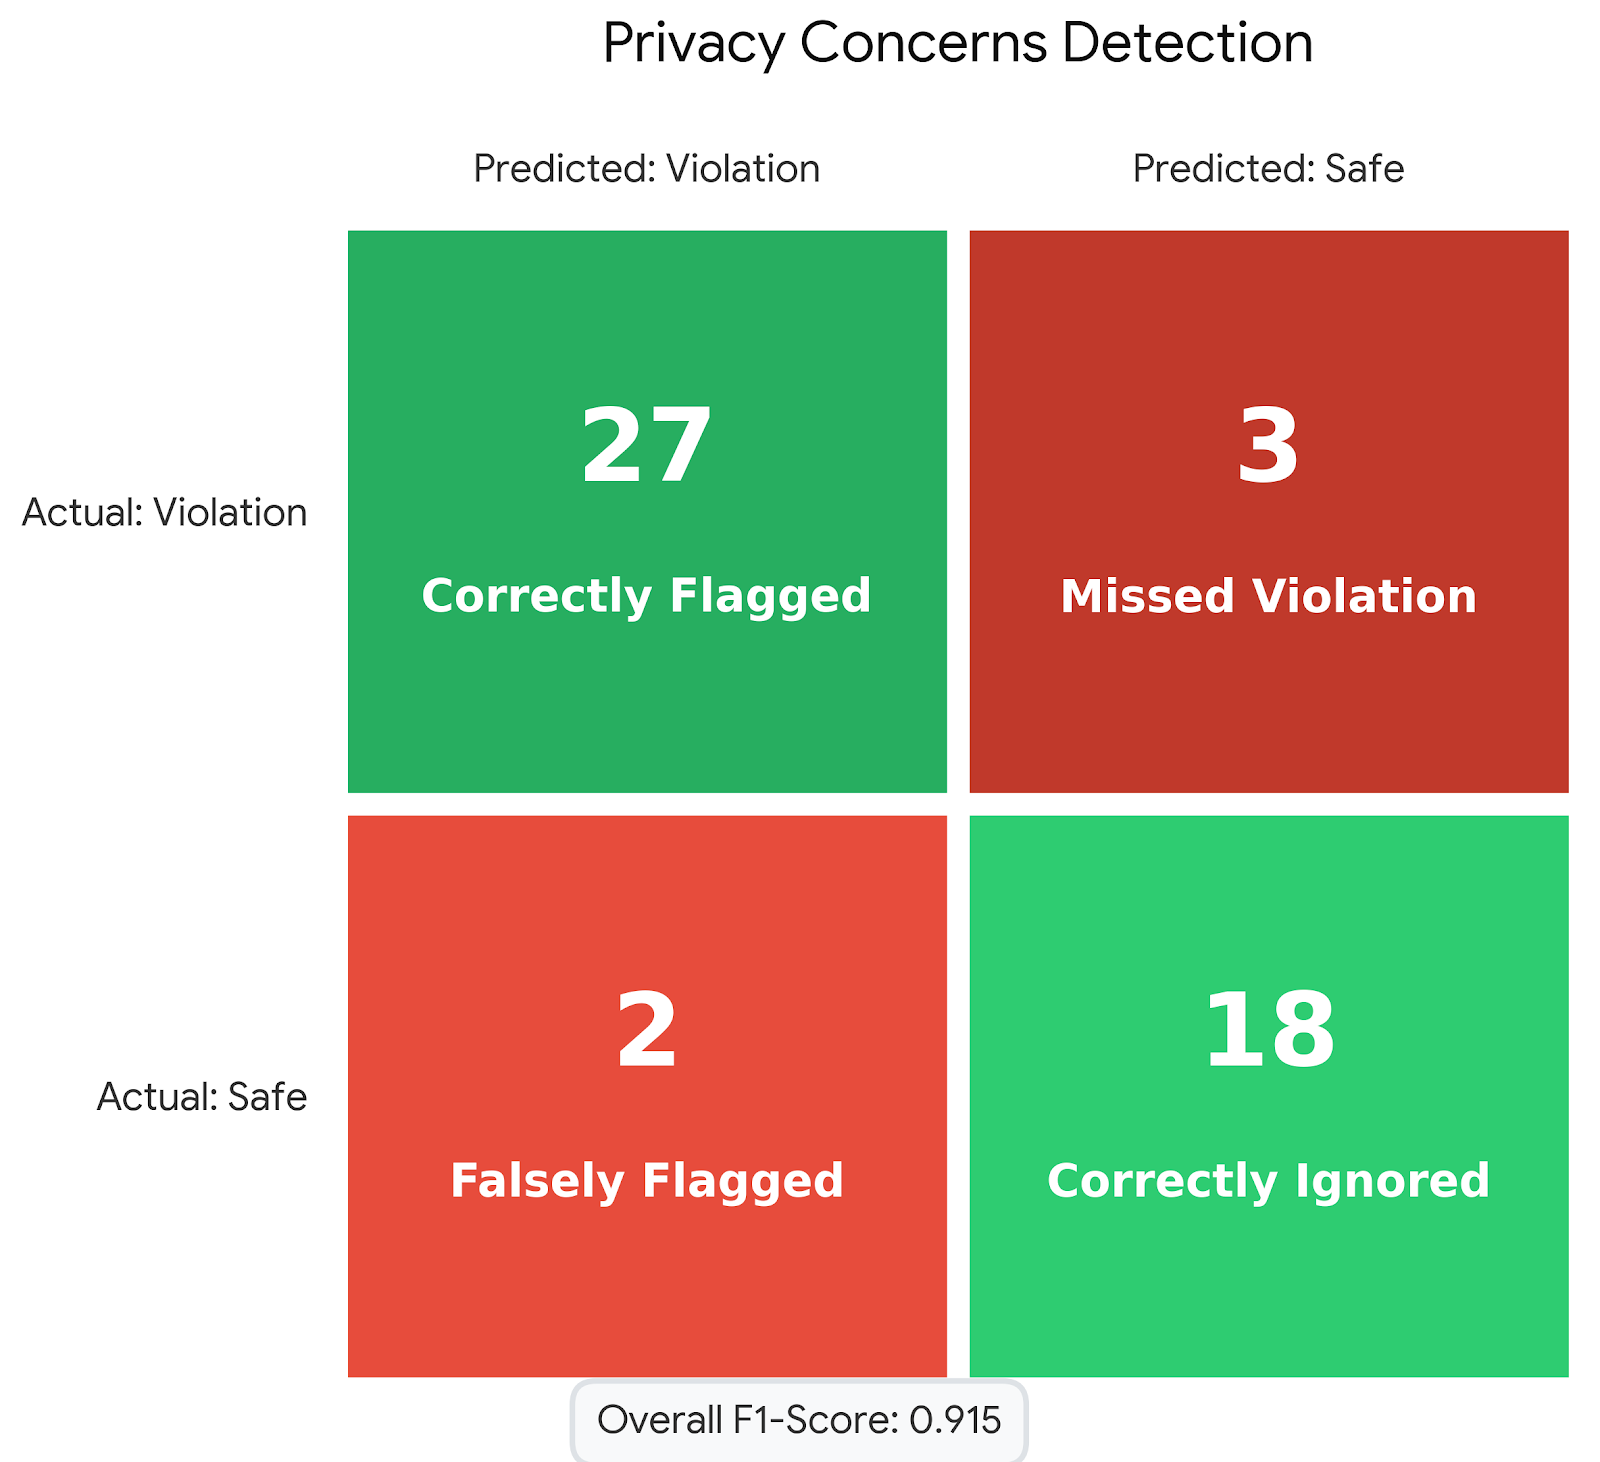
\includegraphics[width=\columnwidth]{img/Confusion-Matrix.png}}
\caption{Detection outcomes per ethical category across 150 test conversations. Each quadrant shows the count of correctly flagged (TP), falsely flagged (FP), missed (FN), and correctly ignored (TN) cases.}
\label{fig:confusion}
\end{figure}

Privacy was the easiest category. Names, addresses, and medical details all have clear textual signals and Gemini caught most of them. Confirmation bias detection also worked well, because the structure of a sycophantic exchange (user states opinion, assistant agrees) is recognizable.

Misinformation was the weakest spot, with an 18\% false positive rate. Gemini sometimes flagged statements that were actually correct, and other times missed claims that were wrong but plausible-sounding. We suspect this will improve as the underlying model improves, but for now, misinformation results need to be taken with some skepticism.

\subsection{Pattern learning}

The weighted learning worked roughly as we hoped. We ran ten sessions simulating a recruiter who kept asking the assistant to help screen candidates. The detection weight for employment discrimination patterns climbed from 6.0 to 8.7 over those sessions. By session seven or eight, the system was catching subtle age and gender bias in job description language that it had missed entirely in session one.

Whether this generalizes to other domains we do not yet know. Our testing was limited.

\begin{figure}[htbp]
\centerline{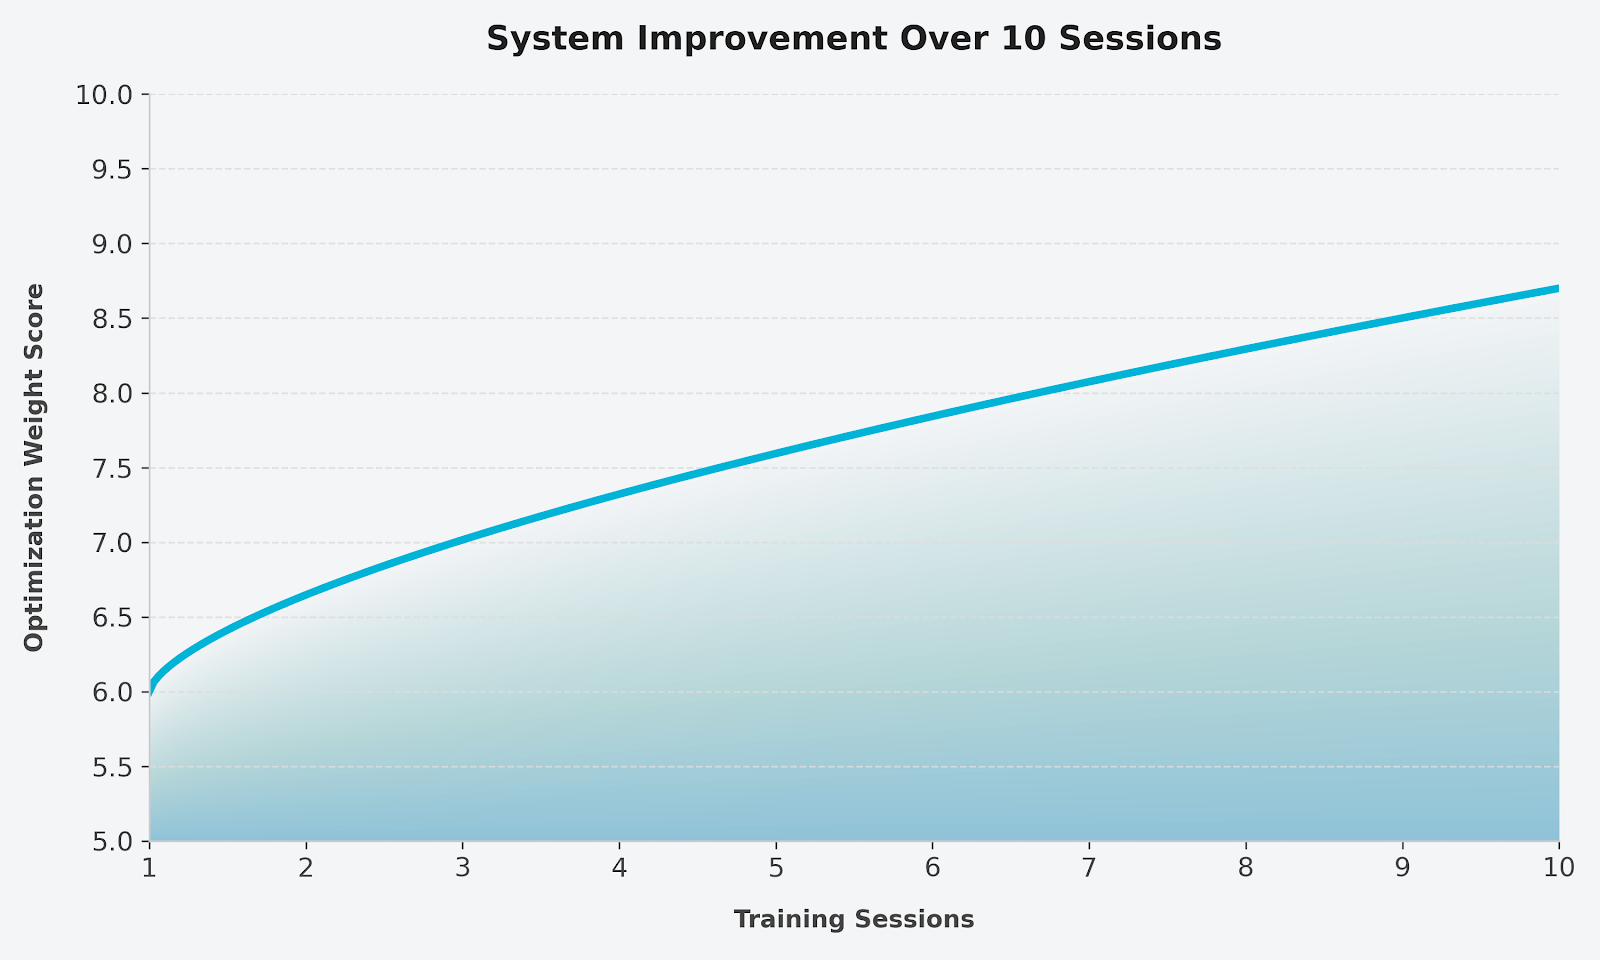
\includegraphics[width=\columnwidth]{img/Line-chart.png}}
\caption{Pattern weight progression for employment discrimination categories over ten consecutive recruiter sessions. Weight climbs from 6.0 to 8.7 as the system encounters repeated instances of the same bias type.}
\label{fig:learning}
\end{figure}

\subsection{Integration}

Getting Neutralis-AI working with Claude through MCP was surprisingly painless. No changes to the assistant's code. It discovered our tools through the standard listing mechanism and started calling them on its own when conversations seemed sensitive. How often it called them varied; Claude appeared to use some internal heuristic we could not inspect. Sometimes it called the ethics tool on benign conversations, and sometimes it skipped it on conversations where we thought it should have triggered.

This unpredictability is a real limitation. We have no control over when the assistant decides to ask for an ethics check.

\subsection{Latency}

Each call to Gemini added 1.5 to 4 seconds of latency, depending on how much context we sent. For conversational use, this felt acceptable. Nobody complained about response times during testing. The round-robin key rotation kept us from hitting rate limits during longer sessions.

\begin{figure}[htbp]
\centerline{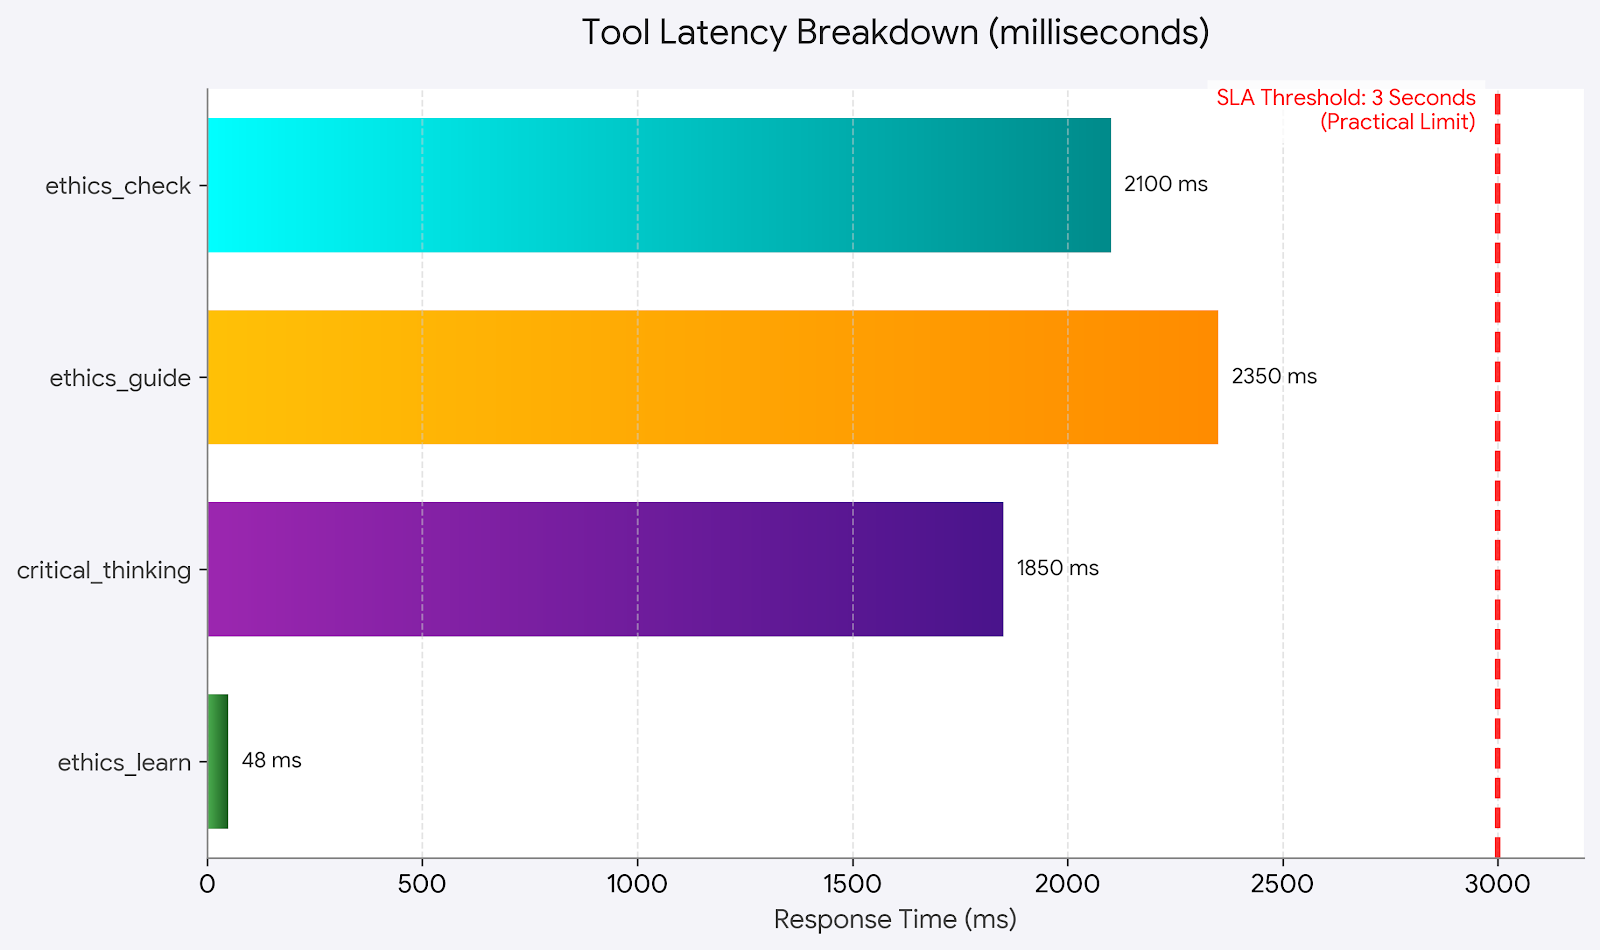
\includegraphics[width=\columnwidth]{img/Latency-Bar-chart.png}}
\caption{Average response latency per tool across 50 test calls. \texttt{ethics\_learn} makes no Gemini API call and runs in under 100\,ms. All AI-backed tools stay within the 4-second ceiling observed during testing.}
\label{fig:latency}
\end{figure}

\subsection{What does not work}

The biggest weakness is the dependency on Gemini. If Gemini misunderstands the context, the analysis will be wrong, and there is no fallback. We saw this happen with culturally specific ethical questions where the model lacked background knowledge.

The pattern memory lives in RAM and disappears when the server restarts. Anything the system learned is gone. This is the most requested fix from people who have tried the system.

There is also a circularity problem we have not solved. We are using an AI model to check another AI model's ethics. Gemini has its own biases, inherited from its training data, and those biases will show up in the ethical analysis. We do not currently audit the auditor.

\section{Future Work}

The most urgent improvement is persistent storage for the pattern memory. Right now, restarting the server erases everything the system has learned. We plan to add a lightweight database backend so learned weights survive across sessions.

Beyond that, we want to support multiple analysis backends. Running the same conversation through both Gemini and a second model would let us cross-check results and reduce the risk of single-model blind spots. A configurable sensitivity slider would also help: different teams have different tolerance for false positives, and right now the threshold is hardcoded.

We have discussed a ``proactive mode'' where the server monitors all messages instead of waiting to be called. We are not sure this is a good idea. It would catch more, but it also starts to look like surveillance, and we are uncomfortable with that tradeoff. For now, we are leaving it to the assistant to decide when to call us.

\section{Conclusion}

You can add ethical oversight to AI conversations without touching the assistant itself. The MCP protocol makes this possible: build a server, register your tools, and the assistant will call them when it thinks they are relevant.

Neutralis-AI is our attempt at doing this. It works well enough to catch real problems that would otherwise slip through. It also misses things, adds latency, and relies on a model that has its own biases. We do not think it is a complete solution. But we think conversations where someone occasionally says ``hold on, have you thought about this?'' are better than conversations where nobody does.

\section*{Acknowledgment}

We built this using Google's Gemini API and Anthropic's Model Context Protocol SDK. Thanks to the open-source contributors who maintain the MCP tooling.

\begin{thebibliography}{00}
\bibitem{b1} A. Perez, S. Ringer, K. Luko\v{s}i\={u}t\.{e}, K. Nguyen, E. Chen, S. Heiner, C. Pettit, C. Olsson, S. Kundu, S. Kadavath, A. Jones, A. Chen, B. Mann, B. Israel, B. Seethor, C. McKinnon, C. Olah, D. Yan, D. Amodei, D. Amodei, T. Henighan, and J. Clark, ``Discovering language model behaviors with model-written evaluations,'' \textit{arXiv preprint arXiv:2212.09251}, 2022.
\bibitem{b2} E. Perez, S. Ringer, K. Luko\v{s}i\={u}t\.{e}, K. Nguyen, E. Chen, and S. Heiner, ``Towards understanding sycophancy in language models,'' in \textit{Proc. ICML Workshop on Challenges in Deployable Generative AI}, 2023.
\bibitem{b3} M. Sharma, M. Tong, T. Korbak, D. Duvenaud, A. Askell, S. R. Bowman, N. Cheng, E. J. Durmus, Z. Hatfield-Dodds, S. R. Johnston, S. Kravec, T. Maxwell, S. McCandlish, K. Ndousse, O. Rauber, N. Schiefer, D. Yan, M. Zhang, and E. Perez, ``Towards understanding sycophancy in language models,'' \textit{arXiv preprint arXiv:2310.13548}, 2023.
\bibitem{b4} L. Floridi and J. Cowls, ``A unified framework of five principles for AI in society,'' \textit{Harvard Data Science Review}, vol. 1, no. 1, 2019.
\bibitem{b5} A. Jobin, M. Ienca, and E. Vayena, ``The global landscape of AI ethics guidelines,'' \textit{Nature Machine Intelligence}, vol. 1, no. 9, pp. 389--399, 2019.
\bibitem{b6} R. K. E. Bellamy, K. Dey, M. Hind, S. C. Hoffman, S. Houde, K. Kannan, P. Lohia, J. Martino, S. Mehta, A. Mojsilovi\'{c}, S. Nagar, K. N. Ramamurthy, J. Richards, D. Saha, P. Sattigeri, M. Singh, K. R. Varshney, and Y. Zhang, ``AI Fairness 360: An extensible toolkit for detecting and mitigating algorithmic bias,'' \textit{IBM Journal of Research and Development}, vol. 63, no. 4/5, pp. 4:1--4:15, 2019.
\bibitem{b7} J. Wexler, M. Pushkarna, T. Bolukbasi, M. Wattenberg, F. Vi\'{e}gas, and J. Wilson, ``The What-If Tool: Interactive probing of machine learning models,'' \textit{IEEE Transactions on Visualization and Computer Graphics}, vol. 26, no. 1, pp. 56--65, 2020.
\bibitem{b8} Anthropic, ``Model Context Protocol documentation,'' 2024. [Online]. Available: \url{https://modelcontextprotocol.io}
\end{thebibliography}

\end{document}
